%Autor: Héctor Fernando Carrera Soto
%Correo: hfcarrerasoto.usac@gmail.com
%Universidad de San Carlos
%Ingeniería electrónica

%%%%%%%%%%%%%%%%%
%	Preámbulo	%
%%%%%%%%%%%%%%%%%

\documentclass[12pt,letterpaper]{article}

\usepackage[left=1.5cm,right=1.5cm,top=1.5cm,bottom=1.5cm]{geometry}

\usepackage{dcolumn}% Align table columns on decimal point
\usepackage{bm}% bold math
%
%Paquete de Idioma
\usepackage[spanish]{babel}
%
%Codificación Alfabeto
\usepackage[utf8]{inputenc}
%
%Codificación de Fuente
\usepackage[T1]{fontenc}
%
%Índice
\usepackage{makeidx}
%
%Gráficos
\usepackage{graphicx}
\usepackage{subfig}
%\usepackage{xcolor} 
%
%Matemática
\usepackage{amsmath}
\usepackage{amsfonts}
\usepackage{amssymb}
%\usepackage{amstext} 
%
%Estilo de Página Numeración superior
%\pagestyle{headings}
%
%Hiperlinks \href{url}{text}
\usepackage[pdftex]{hyperref}
%
%Graficos y tablas
\usepackage{multirow}
%\usepackage{multicol}

%El paquete float es importante para las imágenes con la opción [H] para que las imágenes se coloquen en donde lo deseamos
\usepackage{float}
\usepackage{booktabs}
%
\decimalpoint
%\bibliographystyle{IEEEtran}
%\bibliography{IEEEabrv,mybibfile}
%Para tachar dimencionales
\usepackage{cancel}
%
%%<<<<<<<<<<<<<<<<<<<<  >>>>>>>>>>>>>>>>>>>
%<<<<<<<<<<<<<<<<<<<<  >>>>>>>>>>>>>>>>>>>
%<<<<<<<<<<<<<<<<<<<<  >>>>>>>>>>>>>>>>>>>
%	  Paquetes agregados al formato
%<<<<<<<<<<<<<<<<<<<<  >>>>>>>>>>>>>>>>>>>
%<<<<<<<<<<<<<<<<<<<<  >>>>>>>>>>>>>>>>>>>
%<<<<<<<<<<<<<<<<<<<<  >>>>>>>>>>>>>>>>>>>


%<<<<<<<<< Comando valores absolutos |x| >>>>>
\newcommand{\abs}[1]{\lvert#1\rvert}
%<<<<<<<<< Comando para la normal ||x|| >>>>>
\newcommand{\norm}[1]{\lVert#1\rVert}

%<<<<<<<<< para saltos de página usar  \clearpage >>>>>
%<<<<<<<<< para saltos entre líneas usar \vspace{2cm}>>>>>
%<<<<<<<<< para espaciado horizontal \hspace{1cm}>>>>>
%<<<<<<<<< para colocar url o referencias a url usar \url{http://www.latex-project.org/} o  \href{http://www.latex-project.org/}{latex project}>>>>>>>

%<<<<<<<<<<<<<<<<<<<<  >>>>>>>>>>>>>>>>>>>

%Paquete para configurar medidas de las tablas
\usepackage{tabularx}
%Forma del comando
%\begin{tabular}{|m{0.22\linewidth}|m{0.22\linewidth}|}


%<<<<<<<<< Para configurar \begin{enumerate}[A)]  en donde está la letra "A" escogemos como queremos enumerar, ejemplo \begin{enumerate}[i)]>>>>>>>>>>>>>>

\usepackage{enumerate}

%<<<<<<<<< Cambiar columnas >>>>>

%Se aconseja colocar el documento a una columna y luego cambiarle con forme se vaya utilizando. comandos:
%\begin{multicols}{2}
	%contenido
%\end{multicols}
\usepackage{multicol} %Paquete cambiar columnas

%<<<<<<<<<<<<<<<<<<<<  >>>>>>>>>>>>>>>>>>>

%Configurar sangría
\setlength{\parindent}{0.75cm}

%>>>>>>>>>>>>>>>>>>Esto es para interlineado V2<<<<<<<

%Para interlineado
\renewcommand{\baselinestretch}{1.5}

%Para cambiar la sangría 2
%\setlength{\parindent}{4em}

%Espaciado entre parrafos
%\setlength{\parskip}{1em}

%Separación entre columnas

%Con una línea en medio

%\setlength\columnseprule{1pt}

%Sin una línea en medio

\setlength\columnsep{1.5cm}

%<<<<<<<<<<<<<<<<<<<<  >>>>>>>>>>>>>>>>>>>

%Para colocar punto decimal en lugar de coma automático.
\spanishdecimal{.}

%Para colocar anotaciónes al pié de página, podemos utilizar \footnote{Anotación pié de página}, pegado a la palabra a la cuál se hará la anotación.

%<<<<<<<<<<<<<<<<<<<<  >>>>>>>>>>>>>>>>>>>

%Para agregar un índice: \tableofcontents



%<<<<<<<<<<<<<<<<<<<<  >>>>>>>>>>>>>>>>>>>

% El comando \ balance se puede utilizar para equilibrar las columnas en la página final si se desea. Debe colocarse en cualquier lugar dentro de la primera columna de la última página.
\usepackage{balance}

%\balance
%<<<<<<<<<<<<<<<<<<<<  >>>>>>>>>>>>>>>>>>>

%Use el paquete pdfpages.
%Para incluir todas las páginas en el archivo PDF:
% \includepdf[pages=-]{myfile.pdf}

%Para incluir solo la primera página de un PDF:
%\includepdf[pages={1}]{myfile.pdf}

%Ejecute texdoc pdfpages en un Shell para ver el manual completo de pdfpages.

\usepackage{pdfpages}

%<<<<<<<<<<<<<<<<<<<<  >>>>>>>>>>>>>>>>>>>

%Este comando sirve para importar archivos txt.

\usepackage{verbatim}

% Usar \verbatiminput{archivo.tex}



%<<<<<<<<<<<<<<<<<<<<  >>>>>>>>>>>>>>>>>>>
%Para agregar una caratula más personalizada
%\begin{titlepage}
%	*
%\begin{titlepage}

%<<<<<<<<<<<<<<<<<<<<  >>>>>>>>>>>>>>>>>>>

%Para agregar texto entre ecuaciónes
%\textup{•}
%<<<<<<<<< Permite poner varios autores >>>>>>>>>>>>>

\usepackage{authblk}

%\author[1]{Author \thanks{correo1•university.edu}}
%\author[1]{Author \thanks{correo2•university.edu}}
%\author[1]{Author \thanks{correo3•university.edu}}
%\author[2]{Author \thanks{correo3•university.edu}}
%\author[2]{Author %\thanks{correo4•university.edu}}

%\affil[1]{Department of Computer Science, \LaTeX\ University}
%\affil[2]{Department of Mechanical Engineering, \LaTeX\ University}

%<<<<<<<<<<<<<<<<<<<<  >>>>>>>>>>>>>>>>>>>
%<<<<<<<<<<<<<<<<<<<<  >>>>>>>>>>>>>>>>>>>

%>>>>>>>>>>>>>><Fuente parecido al arial<<<<<<<<<<<
\usepackage{helvet}
\renewcommand*\familydefault{\sfdefault}


\usepackage{apacite}
\begin{document}
%%%%%%%%%%%%%%%%%%%%%%%%%%%%%%%%%%%%%%%%%%%%%%%%%%%%%
%	Cambiando nombre de referencias a bibliografía	%
%%%%%%%%%%%%%%%%%%%%%%%%%%%%%%%%%%%%%%%%%%%%%%%%%%%%%

%Cambiando el nombre de los cuadros y referencias a:
%Tabla y bibliografía

%Cambiando Referencia por Bibliografía
\renewcommand{\refname}{Bibliografía}
%Cambiando Cuadro por tabla
\renewcommand{\tablename}{Tabla}
%Cambiando enumeración arábica a romana en figuras
\renewcommand{\thefigure}{\roman{figure}}
%Cambiando enumeración arábica a romana en tablas
\renewcommand{\thetable}{\roman{table}}

%%%%%%%%%%%%%%%%%
%	Caratula	 %
%%%%%%%%%%%%%%%%%


\begin{titlepage}

\begin{flushleft}
Universidad de San Carlos de Guatemala\\
Facultad de ingeniería\\
Escuela de Ciencias\\
Laboratorio de Química General 1\\
\end{flushleft}

\vspace{7 cm}

\begin{center}
\textbf{Práctica \# 4}\\
{\large \textbf{Determinación del porcentaje en volumen de una bebida alcohólica comercial.}}
\end{center}

\vspace{8 cm}

\begin{tabbing}
\hspace{3cm}\=\hspace{9cm}\=\kill
 Nombre: Héctor Fernando Carrera Soto\>   \> Registro Académico: 201700923\\ 
 Instructor: María Alejandra Escobar Zapeta\>   \> Sección de Laboratorio: P1\\ 
 Fecha de realización: 06/09/2022\>   \> Fecha de Entrega: 20/09/2022
\end{tabbing} 

\end{titlepage}

%%%%%%%%%%%%%%%%
%	Resumen	%
%%%%%%%%%%%%%%%%

%El resumen debe estar dividido en tres párrafos, respondiendo a las siguientes interrogantes:

%<<<<<<<<<<<<<<<<<<<<  >>>>>>>>>>>>>>>>>>>

%¿Qué se hizo?


%<<<<<<<<<<<<<<<<<<<<  >>>>>>>>>>>>>>>>>>>
%¿Cómo se hizo?


%<<<<<<<<<<<<<<<<<<<<  >>>>>>>>>>>>>>>>>>>
%¿A qué se llegó y bajo qué condiciones?


%Todas las interrogantes deben referirse al reporte y no a lo realizado en el Laboratorio, a excepción de algún procedimiento que pudo haber influido sobre los resultados y las condiciones de trabajo. Recuerda que no se colocan las interrogantes, únicamente se contestan a ellas en los párrafos referidos.

%%%%%%%%%%%%%%%%%%%%%
%	Resultados	%
%%%%%%%%%%%%%%%%%%%%%

\section{Resultados}

%Todos resultados deben ser presentados únicamente en tablas. Gráficos sólo serán reportados cuando se te solicite, de lo contrario no colocar gráficos. Las tablas se nombrarán como Tabla 1.\

%Nombre de la tabla. según sea el caso; y los gráficos como Figura 1. Nombre de la figura. según sea el caso. Recordar que desde esta sección se inicia a numerar y nombrar tablas y figuras (gráficos).

%Es importante que puedas agrupar tu información en la cantidad de tablas que consideres necesarias, pero debes cumplir con los objetivos de la práctica.

%%%%%%%%%%%%%%%%%%%%%%%%%%%%%%%%%%%
%	Interpretación de resultados	%
%%%%%%%%%%%%%%%%%%%%%%%%%%%%%%%%%%%

\section{Interpretación de resultados}

%Para la interpretación de resultados debes colocar un párrafo por cada tabla y/o por cada figura que aparezca en la sección de Resultados.

%Recuerda que en esta sección debes cuestionar los resultados obtenidos, no describirlos.

%Tu interpretación dependerá de cuánta información leíste acerca de la temática del reporte.

%No debes colocar teoría directamente, debes utilizarla como respaldo de tus resultados y así poderlos cuestionar, pues esta área no es una investigación.

%%%%%%%%%%%%%%%%%%%%
%	Conclusiones	%
%%%%%%%%%%%%%%%%%%%%

\section{Conclusiones}

%Las conclusiones deben ser concretas y específicas. Estas se realizan en función de los objetivos de la práctica.

%%%%%%%%%%%%%%%%%%%%%%%%%%%%%%
%	Metodología experimental	%
%%%%%%%%%%%%%%%%%%%%%%%%%%%%%%

\section{Metodología experimental}

%Los pasos que se hicieron para realizar la práctica, todo en pasado.



%%%%%%%%%%%%%%%%%%%%%%%%%%%%%%%%%
%	Hoja de datos originales	%
%%%%%%%%%%%%%%%%%%%%%%%%%%%%%%%%%

\section{Hoja de datos originales}


%Use el paquete pdfpages.
%Para incluir todas las páginas en el archivo PDF:
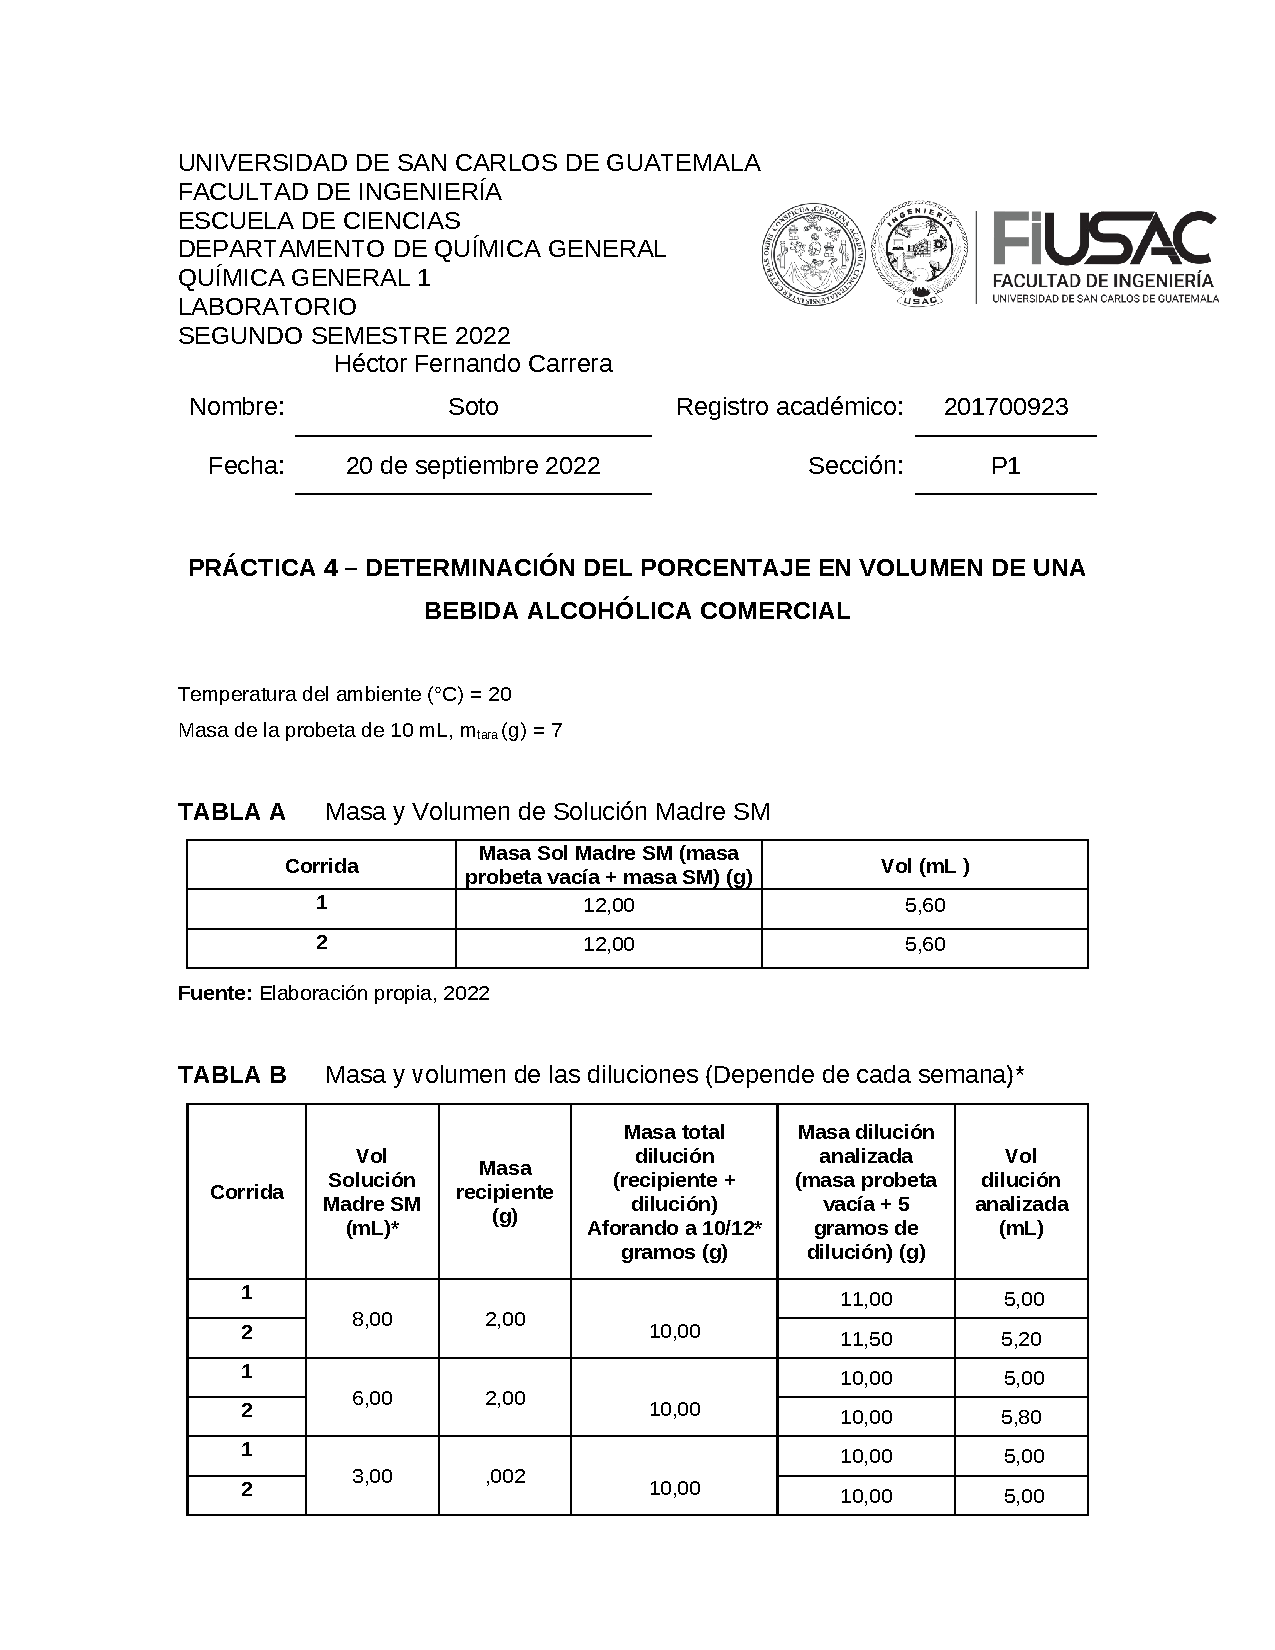
\includepdf[pages=1-2]{HDO.pdf}

%Para incluir solo la primera página de un PDF:
%\includepdf[pages={1}]{myfile.pdf}




%%%%%%%%%%%%%%%%%%%%%%%%%
%	Muestra de cálculo	%
%%%%%%%%%%%%%%%%%%%%%%%%%

\section{Muestra de cálculo}

%En esta sección se deben incluir todos los cálculos del reporte, a excepción de cálculos de Análisis de Error, entre los que se pueden mencionar Error Relativo y Absoluto, Desviación Estándar, Q de Dixon , Límites de Confianza, entre otros.

%Solo debes colocar un ejemplo por cada ecuación que aparezca en esta sección. Por ejemplo si la ecuación de la media o promedio la utilizaste en varios casos (mediciones de masa, de temperatura, tiempo, etc.) solo debes colocar un ejemplo. Para ecuaciones de estadística de medidas de tendencia central (media, desviación estándar, varianza, Q de Dixon, entre otros) utiliza las ecuaciones genéricas, como en el ejemplo 6.3.1 de la Figura 5.

\begin{enumerate}

	\item[1.] Para el porcentaje en volumen $\% \ \frac{V}{V} \ (\%)$, para una solución obtenemos:
%\end{enumerate}

\begin{align}
\% \ \dfrac{V}{V} &= \dfrac{V_{slt}}{V_{slc}} * 100,00
\label{Eq:V_slt/V_slc}\\
V_{slc} &= V_{slt} + V_{slv}
\label{Eq:V_slc}
\end{align}

Sustituyendo la ecuación \ref{Eq:V_slc} en la ecuación \ref{Eq:V_slt/V_slc} podemos describir la ecuación como:

\begin{equation}
\% \ \dfrac{V}{V} = \dfrac{V_{sol}}{V_{sol} + V_{sol}} * 100,00
\label{Eq:V/V}
\end{equation}

Dónde:\

$\% \ \dfrac{V}{V}$: Porcentaje en volumen.\

$V_{slt}$: Volumen de soluto.\

$V_{slv}$: Volumen de solvente.\

$V_{slc}$: Volumen de la solución.

\end{enumerate}


%%%%%%%%%%%%%%%%

\begin{enumerate}

	\item[2.] Para el cálculo de la densidad de las soluciónes podemos describir la ecuación como:
%\end{enumerate}

\begin{align}
\rho &= \dfrac{m_{slc}}{V_{slc}}
\label{Eq:Densidad_slc}\\
m_{slc} &= m_{slt} + m_{slv}
\label{Eq:Masa_slc}
\end{align}

Sustituyendo las ecuaciónes \ref{Eq:Masa_slc} y \ref{Eq:V_slc} en la ecuación \ref{Eq:Densidad_slc}, obtenemos:

\begin{equation}
\rho = \dfrac{m_{slt} + m_{slv}}{V_{slt} + V_{slv}}
\label{Eq:rho}
\end{equation}

Dónde:\

$\rho$: Densidad del soluto.\

$V_{slt}$: Volumen de soluto.\

$V_{slv}$: Volumen de solvente.\

$V_{slc}$: Volumen de la solución.\

$m_{slt}$: Masa de soluto.\

$m_{slv}$: Masa de solvente.\

$m_{slc}$: Masa de la solución.

\end{enumerate}


%%%%%%%%%%%%%%%%%%%%%%%%%
%	Análisis de Error	%
%%%%%%%%%%%%%%%%%%%%%%%%%

\section{Análisis de Error}

%Análisis de Error En esta sección se colocarán todos cálculos de Error Relativo, Error Absoluto, Desviación Estándar, Q de Dixon, Límites de Confianza, entre otros. Además se incluirá una tabla de las incertezas de los instrumentos y equipo utilizado para realizar la práctica.

%El Análisis de Error es prácticamente una Muestra de Cálculo, con la diferencia que en esta sección se colocan los cálculos mencionados anteriormente.


\begin{enumerate}
	\item[3.] Determinación de la media para datos necesarios en los cálculos.
	
\begin{equation}
\overline{X_{k}} = \dfrac{\Sigma_{i=1}^{n} (x_{i})}{n}
\label{Eq:Media}
\end{equation}	

Dónde:\

$\overline{X_{k}}$: Media de los datos adquiridos o cálculados.\

$x_{i}$: Datos a los que se les desea calcular la media.\

$n$: Número de datos adquiridos de cada corrida.
	
\end{enumerate}

Utilizando los datos tabla \ref{Tab:Media}, calculados con la ecuación número \ref{Eq:V/V}, obtenemos:\

\begin{align*}
\overline{X_{\% \ V/V}} &= \dfrac{a+b+c}{3,00}\\
\overline{X_{\% \ V/V}} &=
\end{align*}

%%%%%%%%%%%%%%%%%%%%%%%%%%%%%%%%%%%%%%%%%%%%
%%%%%%%%%%%%%%%%%%%%%%%%%%%%%%%%%%%%%%%%%%%%

\begin{enumerate}
\item[4.] Determinación de la desviación estándae del $\% \ \frac{V}{V} \ (\%)$ de la solución.

\begin{equation}
\sigma = \sqrt{\dfrac{\Sigma_{i=1}^{n}(\% \ \dfrac{V}{V} - \overline{X_{\% \ V/V}})^{2,00}}{n-1,00}}
\label{Eq:Desv}
\end{equation}

Dónde:\

$\sigma$: Desviación estándar del $\% \ \frac{V}{V} \ (\%)$.\

$\overline{X_{\% \ V/V}}$: Media de la densidad del $\% \ \frac{V}{V} \ (\%)$.\

$\% \ \dfrac{V}{V}$: Porcentaje en volumen.\

$n$: Número de datos adquiridoa para el $\% \ \frac{V}{V} \ (\%)$ de cada corrida.

\end{enumerate}

Utilizando la ecuación número \ref{Eq:Desv}, \ref{Eq:Media} y \ref{Eq:Densidad}, obtenemos que la desviación estándar es de:

\begin{align*}
\sigma &= \sqrt{\dfrac{(a - x)^{2,00} + (b - x)^{2,00} + (c - x)^{2,00}}{3,00-1,00}}\\
\sigma &= 0
\end{align*}

%%%%%%%%%%%%%%%%%%%%%%%%%%%%%%%%%%%%%%%%%%%%
%%%%%%%%%%%%%%%%%%%%%%%%%%%%%%%%%%%%%%%%%%%%

\begin{enumerate}
	\item[5.] Determinación del porcentaje de error absoluto de la densidad, tomando como densidad experimental, la densidad media calculada con la ecuación número \ref{Eq:Media}.
	
\begin{equation}
\% Er_{abs} = \abs{\rho_{exp} - \rho_{teo}}*100,00
%\label{Eq:Error_abs}
\end{equation}

$\% Er_{abs}$: Error absoluto de la densidad.\\

$\rho_{exp}$: Densidad experimental.\\

$\rho_{teo}$: Densidad teórica.

\end{enumerate}

Sustituyendo datos en la ecuación \ref{Eq:Error_abs} se obtiene:

\begin{align*}
\% Er_{abs} &= \abs{2,06 - 1,93}*100,00\\
\% Er_{abs} &= 13,15 \%
\end{align*}

%%%%%%%%%%%%%%%%%%%%%%%%%%%%%%%%%%%%%%%%%%%%
%%%%%%%%%%%%%%%%%%%%%%%%%%%%%%%%%%%%%%%%%%%%

\begin{enumerate}
	\item[8.] Determinación del porcentaje de error relativo de la densidad calculada por medio de arquimides.
	
\begin{equation}
\% Er_{rel} = \dfrac{\abs{\rho_{exp} - \rho_{teo}}*100,00}{\rho_{teo}}
%\label{Eq:Error_rel}
\end{equation}

$\% Er_{rel}$: Error relativo de la densidad.\\

$\rho_{exp}$: Densidad experimental.\\

$\rho_{teo}$: Densidad teórica.

\end{enumerate}

Sustituyendo datos en la ecuación \ref{Eq:Error_rel} se obtiene:

\begin{align*}
\% Er_{rel} &= \dfrac{\abs{2,06 - 1,93}*100,00}{1,93}\\
\% Er_{rel} &= 6,81 \%
\end{align*}

%%%%%%%%%%%%%%%%%%%%%%%%%%
%	Datos calculados 	 %
%%%%%%%%%%%%%%%%%%%%%%%%%%

\section{Datos calculados}

%En esta sección se agrupan en tablas y de forma ordenada los resultados de todos los cálculos de las secciones Muestra Cálculo y Análisis de Error. No se deben colocar ecuaciones o datos originales en esta sección.

\begin{table}[H]
\begin{center}

\begin{tabular}{|c|c|}
\hline 
\textbf{Volumen cubo} [$\textup{cm}^{3}$] & \textbf{Volumen cilindro} [$\textup{cm}^{3}$] \\ 
\hline 
1,40 & 6,22 \\ 
\hline 
\end{tabular} 

\caption{Volumenes calculados utilizando las medidas obtenidas con la regla.}
\centering{\textbf{Fuente:} Elaboración propia, 2022.}

\label{Tab:vol_regla}
\end{center}
\end{table}






\begin{table}[H]
\begin{center}

\begin{tabular}{|c|c|c|}
\hline 
\textbf{Corrida} & \textbf{Volumen cubo} [$\textup{cm}^{3}$] & \textbf{Volumen cilindro} [$\textup{cm}^{3}$] \\ 
\hline 
1 & 1,00 & 5,5 \\ 
\hline 
2 & 0,50 & 6,00 \\ 
\hline 
3 & 1,40 & 6,00 \\ 
\hline 
\end{tabular} 

\caption{Volumenes calculados utilizando Arquimides.}
\centering{\textbf{Fuente:} Elaboración propia, 2022.}

\label{Tab:vol_arq}
\end{center}
\end{table}




\begin{table}[H]
\begin{center}

\begin{tabular}{|c|c|c|}
\hline 
\textbf{Corrida} & \textbf{Densidad cubo} [$\textup{g} / \textup{cm}^{3}$] & \textbf{Densidad cilindro} [$\textup{g} / \textup{cm}^{3}$] \\ 
\hline 
1 & 2,00 & 2,18 \\ 
\hline 
2 & 4,00 & 2,00 \\ 
\hline 
3 & 2,00 & 2,00 \\ 
\hline 
\end{tabular} 

\caption{Densidades calculados utilizando Arquimides.}
\centering{\textbf{Fuente:} Elaboración propia, 2022.}

\label{Tab:den_arq}
\end{center}
\end{table}





\begin{table}[H]
\begin{center}

\begin{tabular}{|c|c|c|}
\hline 
\textbf{Corrida} & \textbf{Densidad cubo} [$\textup{g} / \textup{cm}^{3}$] & \textbf{Densidad cilindro} [$\textup{g} / \textup{cm}^{3}$] \\ 
\hline 
1 & 1,43 & 1,93 \\ 
\hline 
2 & 1,43 & 1,93  \\ 
\hline 
3 & 1,43 & 1,93  \\ 
\hline 
\end{tabular} 

\caption{Densidades calculados utilizando las dimensiónes de las figuras.}
\centering{\textbf{Fuente:} Elaboración propia, 2022.}

\label{Tab:den_medidas}
\end{center}
\end{table}




\begin{table}[H]
\begin{center}

\begin{tabular}{|c|c|c|}
\hline 
\textbf{Valores medios} & \textbf{Volumen} [$\textup{cm}^{3}$]& \textbf{Densidad} [$\textup{g} / \textup{cm}^{3}$]\\ 
\hline 
\textbf{Cilindro} & 5,83 & 2,06 \\ 
\hline 
\textbf{Paralelepípedo} & 0,83 & 2,67 \\ 
\hline 
\end{tabular} 

\caption{Valores medios del volumen y densidad, calculados por medio de arquímides, de cada figura.}
\centering{\textbf{Fuente:} Elaboración propia, 2022.}

\label{Tab:Media}
\end{center}
\end{table}




\begin{table}[H]
\begin{center}

\begin{tabular}{|m{3cm}|m{3cm}|m{3cm}|m{3cm}|}
\hline 
\textbf{Figura} & \textbf{Error relativo} [$\%$] & \textbf{Error absoluto} [$\%$] & \textbf{Desviación estándar} \\ 
\hline 
\textbf{Paralelepípedo} & 86,67 & 123,81 & 1,16 \\ 
\hline 
\textbf{Cilindro} & 6,81 & 13,15 & 0,11 \\ 
\hline 
\end{tabular} 

\caption{Errores absolutos, relativos y desviación estándar de cada figura.}
\centering{\textbf{Fuente:} Elaboración propia, 2022.}

\label{Tab:Errores}
\end{center}
\end{table}


%%%%%%%%%%%%%%%%%%%%%
%	Bibliografías	%
%%%%%%%%%%%%%%%%%%%%%

%Primero darle a F11, luego a F6 y por último compilamos, así veremos la bibliografía, esto cada vez que hagamos una citación en nuestro documento.

\bibliographystyle{apacite}
\nocite{*} %Descomentar para que genere la bibliografía sin citar
%\cite{Einstein} Para citar al final del parrafo citado.
%\cite[p.10]{Einstein} Para citar al final del parrafo citado con página.
%\nocite{Einstein} Para mostrar en referencias sin citar.
\bibliography{bibliografia}


\end{document}
